%%==========================
%% chapter01.tex for SJTU Master Thesis
%% based on CASthesis
%% modified by wei.jianwen@gmail.com
%% version: 0.3a
%% Encoding: UTF-8
%% last update: Dec 5th, 2010
%%==================================================

%\bibliographystyle{sjtu2} %[此处用于每章都生产参考文献]

% 第四章的布局:
% 整体介绍,附图 1000
% 分块方法,简单分块,滑动块分块?1000
% 对分块预处理,一些复杂的方法,以及缺点 2000
% 预处理完进行FFT变换,分析理论 2000
% 对输出的结果与库中的值做余弦定理,提出\epislon参数 2000
% 加入spark以后算法的架构 2000

\chapter{基于FFT的文件去重算法}
\label{chap:algo}

\section{背景介绍}
\label{sec:back}

在第二章中,已经详细介绍了当今互联网大数据环境下的各种文件去重的核心算法,每一小节介绍算法分别改进和优化了前一小节中的算法并且在效率上有着显著的提升。

这些算法的主要思想是,先将文件分块,作为算法下一步的输入,分块的大小由系统的设定而决定,一般取值为使系统效率最高的那个值,分块的目的是为了更方面下一阶段的处理;接着共同的一步是对文件块进行哈希计算,比如SHA1的哈希值,需要注意的是,MD5也是一个比较好的方案,但是在一般的场景下用SHA1来代替MD5,一个最重要的原因是MD5已经被证明可以进行碰撞攻击。也就是说,攻击者可以产生两个应用程序,内容不一样,但是哈希值完全一样;将输出的SHA1哈希值与服务器上已经保存的哈希值做比较,若有发现符合,则说明这个文件块在服务器上已经有了一份拷贝,需要再次上传和存储;若没有发现符合,则认为这是一份新的文件块,客户端需要上传这份文件块。

在上述的通用算法中,一个很重要的一点是,只能检测两个完全相同的文件是否相同,如果一个文件的任意字节被改动,这两个文件即被视为不相同,即这是一个“零一”问题,要么相同要么不相同,没有中间的可能性。但是一个拥有这种中间可能性的检测算法在某些场景下是非常被需要的,比如若两个文件的文件内容的相似度达到95\%及以上的时候,这两个文件即可被视为相同的文件。一个典型的应用场景是一个新闻报导系统,在这个系统中规定相同内容的报导不能被同时报导两次,即若两条新闻都是关于X和Y关系的主题,系统应该检测出第二条新闻与前一条新闻相似并且予以警告,这个相似度系数可以按照系统的需求而调节,比如某些情况下完全不同的报导才是不一样的报导,这个时候相似度就是100\%,而某些情况下只要90\%内容相同则是相同的报导,本文提出的基于FFT的文件去重算法就是在这样的背景下提出的,这个算法中,有一个系统参数$\epsilon$,可以动态地调节系统对相似度的需求,有很大的灵活性。基于FFT的去重算法的其它部分(分块的选择,分块预处理,FFT变换,对输出进行处理和比较)将在下面的几个小节中一一介绍。

\begin{figure}[!hbp]
%\centering
    \begin{minipage}[b]{0.6\textwidth}
    \captionstyle{\centering}
    \centering
    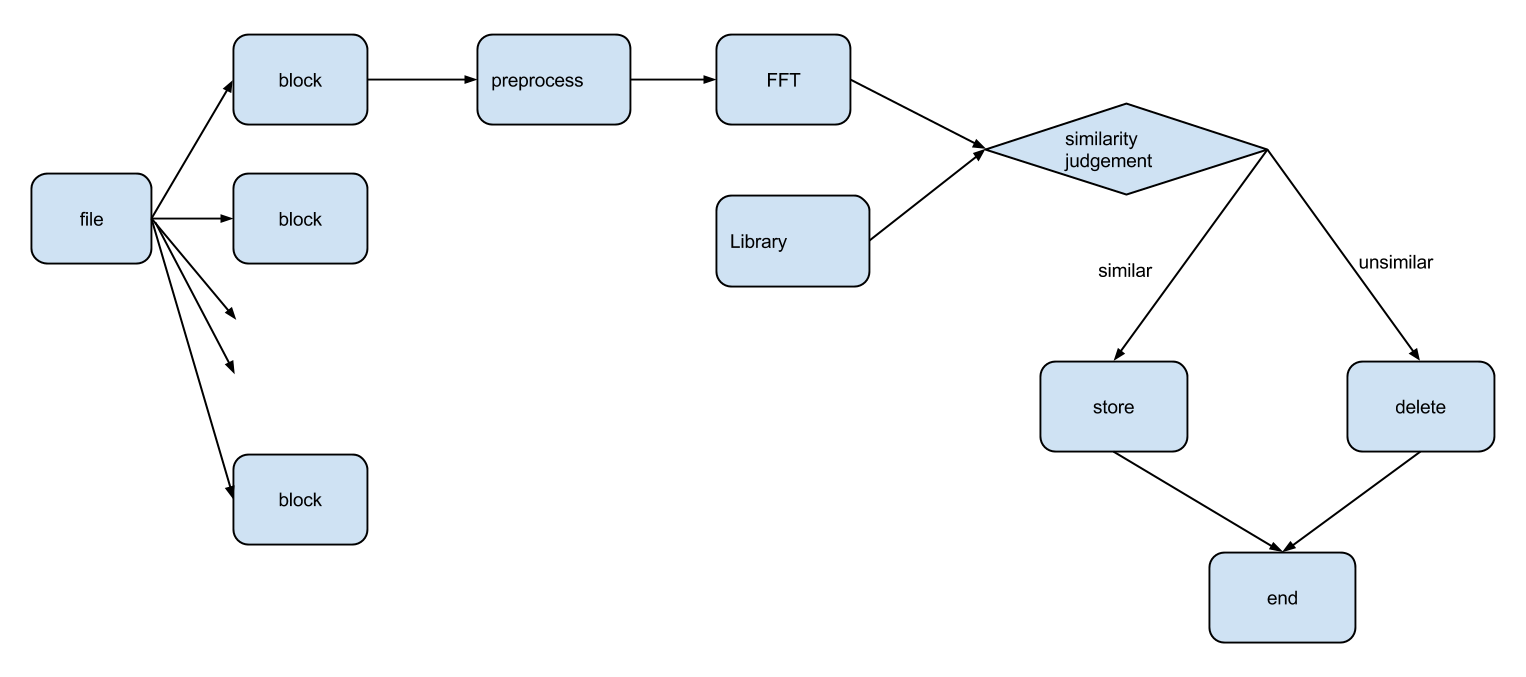
\includegraphics[origin=br,width=18cm]{chap4/archti.png}
    \bicaption[fig:archti]{这里将出现在插图索引}{基于FFT的文件去重算法架构.}{Fig}{Archtecture.}
    \end{minipage}     
\end{figure}

在图\ref{fig:archti}中,简单得描述了这个算法的简要步骤,首先,基于一些方法将一个大文件分成若干个文件块,这个文件块的输入将作为预处理的输出,预处理的输出将作为FFT的输入,FFT的输出是一个N维的向量,此时这个向量就代表了这个文件块,称为文件块的特征向量,与服务器端的库文件进行相似度的测试,此时需要依赖系统参数$\epsilon$,若相似,则不存储;若不相似,则存储,算法结束。本章节将详细介绍每一步骤的算法和设计理念。

\section{分块方法}
\label{sec:choice}

在第二章我们简单地提到过,若使用简单分块的方法,即对任意一个文件按照固定长度的切分成一个个文件块的方法,会遭受到插入问题(insertion problem)和删除问题(deletion problem)的影响导致去重性能急剧下降。简单来说,若采用简单分块的方法,那么边界是由预定义的分块大小决定的,此时如果任意插入或者删除一个字符,那么在这个分块之后的所有分块的内容都会向后或者向前偏移一个字符,导致了这个分块以后的所有分块都不相同,造成的结果是,即使后面的文件块毛无变化,但服务器上还是会存储多分冗余的拷贝。解决这个问题的一个方案是,不采用基于文件块大小作为块划分边界的依据,而是采用另外一种方法,即先定义一个滑动窗口,若文件的某一个滑动窗口满足一定事先约定的条件,那么这个滑动窗口对应的最后一个字节才是这个分块的最后一次字节。采用这种分块方法的好处的是,若随便插入或删除一个字符,那么只会影响当前块和之后的一个块,而其它块均不受影响,大大提高了存储的效率,此时的文件分块不再是以内容长度作为边界的依据值,还是根据内容。在本文基于FFT的文件去重算法中,我们采用简单分块的方式而不是基于滑动窗口的方法,理由主要是以下几点:

\begin{enumerate}
\item 保证了模型的简易性,将重点放在了FFT,余弦定理和系统参数$\epsilon$上
\item 在仿真阶段我们实现系统的主要框架,用简单分块大大简化了原形的实现
\item 本算法的重点并不是分块方法,可以由专门的论文来详细讨论
\end{enumerate}

事实上,若将此算法应用在工业界的实际使用中,那么考虑到存储的效率等等因素,一般还是会采用基于滑动窗口的分块方式,在之后的所有讨论中,将默认采用的时简单分块的大小,即直接将文件通过块的大小分成若干份,在服务器上的所有数据都是以块为单位,一个文件由若干个块组成。

\section{分块预处理}
\label{sec:proproc}

在本章中,将详细讲解分块预处理的必要性以及具体方法和步骤,我们将讨论一个现有的分块预处理的方法,分析这个方法的优缺点,并提出一种简单高效的分块方法。

\subsection{为什么要预处理}
\label{sec:why}

在\ref{fig:archti}中,我们可以看到,当文件分块以后,要经过一个预处理的过程,这一步是十分必要的,它的作用是将不同形式的输出和输入能够非常好地连接在一起,比如复数形式的FFT的输入是一个N维的复数向量,而一个分块是一个文件,它是一个个字节组成的数据,怎么接近无缝地连接这两个模块是十分重要的,在本文中,将详细讨论这个过程。

\subsection{预处理的方法}
\label{sec:appro}

在{参考}中,利用了离散傅里叶变换来解决网页去重,在这个算法中,把每个字符都映射成一个字符,那么每篇网页就可以表示成一个离散的序列$y(i)$,重复的网页应该具有相似的序列,对该序列进行离散傅里叶变换就可以得到傅里叶系数$a_n$和$b_n$,然后通过某种方法比较两个网页文件的傅里叶系数的前几项就可以大致比较出两个网页的相似度。在这篇研究中,预处理的方法主要是将一个字符映射到该字符对应的语义数值。

一个比较合适的字符到语义数值的转化应该满足,语义上相似的字符值对应的语义值应该相近,语义上不相似的字符值对应的语义值应该相差较大。该方法采用了如下方法作为计算每个字符的语义值的方法:以大量互联网上的文本素材作为基础,统计这些文本材料中字符和字符出现的关系,假设不同的字符数为N,那么统计的结果将是一个$N \times N$矩阵,其中$R(i, j)$的值定义为字符i和字符j相邻出现的次数除以字符i在文本素材中出现的总次数,若$i==j$,则这个值被定义为1,于是字符i的语义值就可以由N维向量$R(i)$来表示,但$R(i)$是一个向量,我们需要的是一个数值,也就是说需要对这个N维向量进行降维的操作,在该研究中采用K-L变换(Karhunen-Loeve)的方法对$R(i)$降维,它是一种建立在统计特性基础上的一种转化,目的是将数据做转化,使得转化后数据的相关性最小。基于语义的预处理方法的优点是,这样的预处理方法比较新颖,并且是基于语义的,基于语义的一个最大的好处就是能够非常接近真实地反映原来数据之间的关系,并且能按照这样的关系模拟出一个具体的数值来代表这种关系,在某些基于语义的去重的场景下,这样的算法将非常合适。

实际上,对于互联网上的大数据而言,使用基于语义的预处理意义并不是特别大。首先,通常意义下的去重算法只关心两个文件严格意义上是否相同,即任意字符就代表文件的一个标志位,若这个字符不相同,则两个文件则不相同,而不在意这个字符与下一个字符之间的关系;其次,在上述的描述中我们需要实现构建一个$N \times N$的矩阵,这个矩阵是基于互联网上大量的文本素材所构建的,但是在实际中,这些素材的来源将很大程度上决定了这个$N \times N$矩阵的性质,需要严格保证这些素材的随机性,不仅如此,N将会是一个非常大的数字,表的一部分可能存在磁盘中,导致了一次读取表的操作都可能引起一次潜在的磁盘读取,对于高时效性高性能的大数据计算,这样的延时显然是不允许的。综上,基于语义的算法有很多不足之处,本文将提出一种简易的,可实现的同时具有保真性的预处理算法。

由分析可知,字符和字符之间的语义关系是不会影响两个文件之间相似度的判定,于是在本文中,将直接将文件的每一个字节看作是一个个离散的点,每个点取值范围为0至255,作为输入复数组中每一个复数的实数部分,即若一个1MB的文件经过预处理,则输出的是一个1*1024*1024维的复数向量,其中实部$real(i)=$第i字节对应的值,虚部$imag(i)=0$。这么做的好处有以下几点:

\begin{enumerate}
\item 完全脱离了语义的束缚,把着重点放在了每个字节上;
\item 从抽象角度上,更容易理解怎么把一个文件映射成一个离散的信号,以此作为FFT的输入;
\item 提高设计的简单性,实现的可行性。在仿真阶段,如果采用基于语义的预处理方法,将大大增加仿真的复杂度和难度,首先文本样本的选择是第一个问题,其次对于有些小型机器内存不一定能完全放下,这些在上面已讨论过。
\end{enumerate}

在下一小节说,将详细说明对变换后的文件使用傅里叶变换的意义和具体算法。

\section{对文本进行FFT变换的意义}
\label{sec:ffttr}

从本质上来说,傅里叶变换不仅仅是一个数学工具,更是一种看待事物的一种思维方式,从时域上来讲,一切事物都在变化,换一个角度,若从频域上来讲,好像一切都是事先约定好的,有规律可循的,静止的。本章节将从抽象的角度来阐明怎么把FFT应用在文件去重这个领域上。

对于计算机而言,DFT是唯一能应用的一种傅里叶变换的变体,在数学的推导中,函数可以是连续的,所以有连续傅里叶变换和离散傅里叶变换,但计算机无法处理连续的信号,它只能对连续的信号进行采样,然后处理这些有间隔的离散的点。一个比较常用的例子是,音频信号在时域中显然是连续的,但计算机在记录音频并做处理的时候需要先对音频信号进行采样,两个样本之间会经历一个很小很小的时间$\Delta t$,于是整个音频的信号就可以变成时域上若干离散的点,从而可以进行下一步的处理。

理解傅里叶变换对输入转化的抽象意义是本文的一个难点,为了帮助读者理解对文本进行FFT变换的意义,将先举一个音乐的例子。在没有学习过乐器的人的理解中,音乐就是随时间变化的震动;而在一些乐器玩家的
\section{应用余弦定理}
\label{sec:applycos}

\section{基于spark的算法设计}
\label{sec:spark}
